\documentclass[twoside,11pt]{article}
\usepackage{jmlr2e} 
\usepackage{url,graphicx} 

\jmlrheading{1}{2014}{XX-XX}{5/14}{00/00}{Bouckaert}
\ShortHeadings{BEASTShell}{Bouckaert}

\begin{document}
\title{BEASTShell -- scripting for Bayesian hierarchical clustering}
\author{\name Remco R. Bouckaert \email remco@cs.auckland.ac.nz}
\editor{---}
\maketitle

\begin{abstract}
BEASTShell is a scripting langauge base on BeanShell for scripting BEAST,
a package for Bayesian hierarchical clustering. BEASTStudio is a GUI that 
supports BEASTShell through a shell environment, variable inspector, editors, 
online interactive help and a set of commands and graphical components for 
visualising graphs and tree hierarchies.
This facilitates simulations studies for hierarchical clustering models,
interactive exploration of properties of hierarchies produced by a BEAST 
analysis, flexible extensions of Bayesian hierarchical clustering through 
BEAST Shell scripts and unit tests.

BEASTShell is hosted on GitHub and details on installation can be found at
\url{https://github.com/CompEvol/beastshell}.
\end{abstract}
\begin{keywords}
  hierarchical clustering, MCMC, scripting, GUI, open source
\end{keywords}

\section{Introduction}

BEAST \citep{beast2} is a an open source package writting in Java for Bayesian hierarchical 
clustering. It is popular among biological sciences, e.g for studying moas \citep{bunce2003extreme}
and cholera \citep{mutreja2011evidence} and social sciences, e.g. for language clustering \citep{bouckaert2012mapping,gray2009language}.
A growing number of packages is available\footnote{See the BEAST wiki at
\url{http://www.beast2.org/wiki}}. It uses an architecture for building models that 
relies on the model being a directed acyclic graph. Each object is derived from a BEAST 
Object and BEAST Objects are connected to each other through Inputs -- classes that 
specify properties on incoming edges to a BEAST Object. Figure \ref{fig.model} shows
a fragment of a BEAST model, where the rockets represent BEAST Objects and the thrusters
represent Inputs. This design provides automatic XML generation and parsing, type checking, 
automatically generated GUIs, tooltip information for GUIs, encoding common
rules for inputs (e.g. which ones are required), default values for inputs, etc (see
\cite{beastbook} for more details). Unfortunately, one of the drawbacks this set up
shares with JavaBeans is that the constructor of a BEAST Object can only be called after
all Inputs have been defined. BEAST Objects have the {\tt initAndValidate} method that should be 
called after all Inputs of a BEAST Object have been set. This makes it cumbersome to
initialise BEASTObjects in Java programs, and consequently makes it tedious to perform
tasks like setting up simulations studies and analysing results for a specific hierarchical
clustering analysis. The goal of BEASTShell is to make these tasks easier.

\begin{figure}
\begin{center}
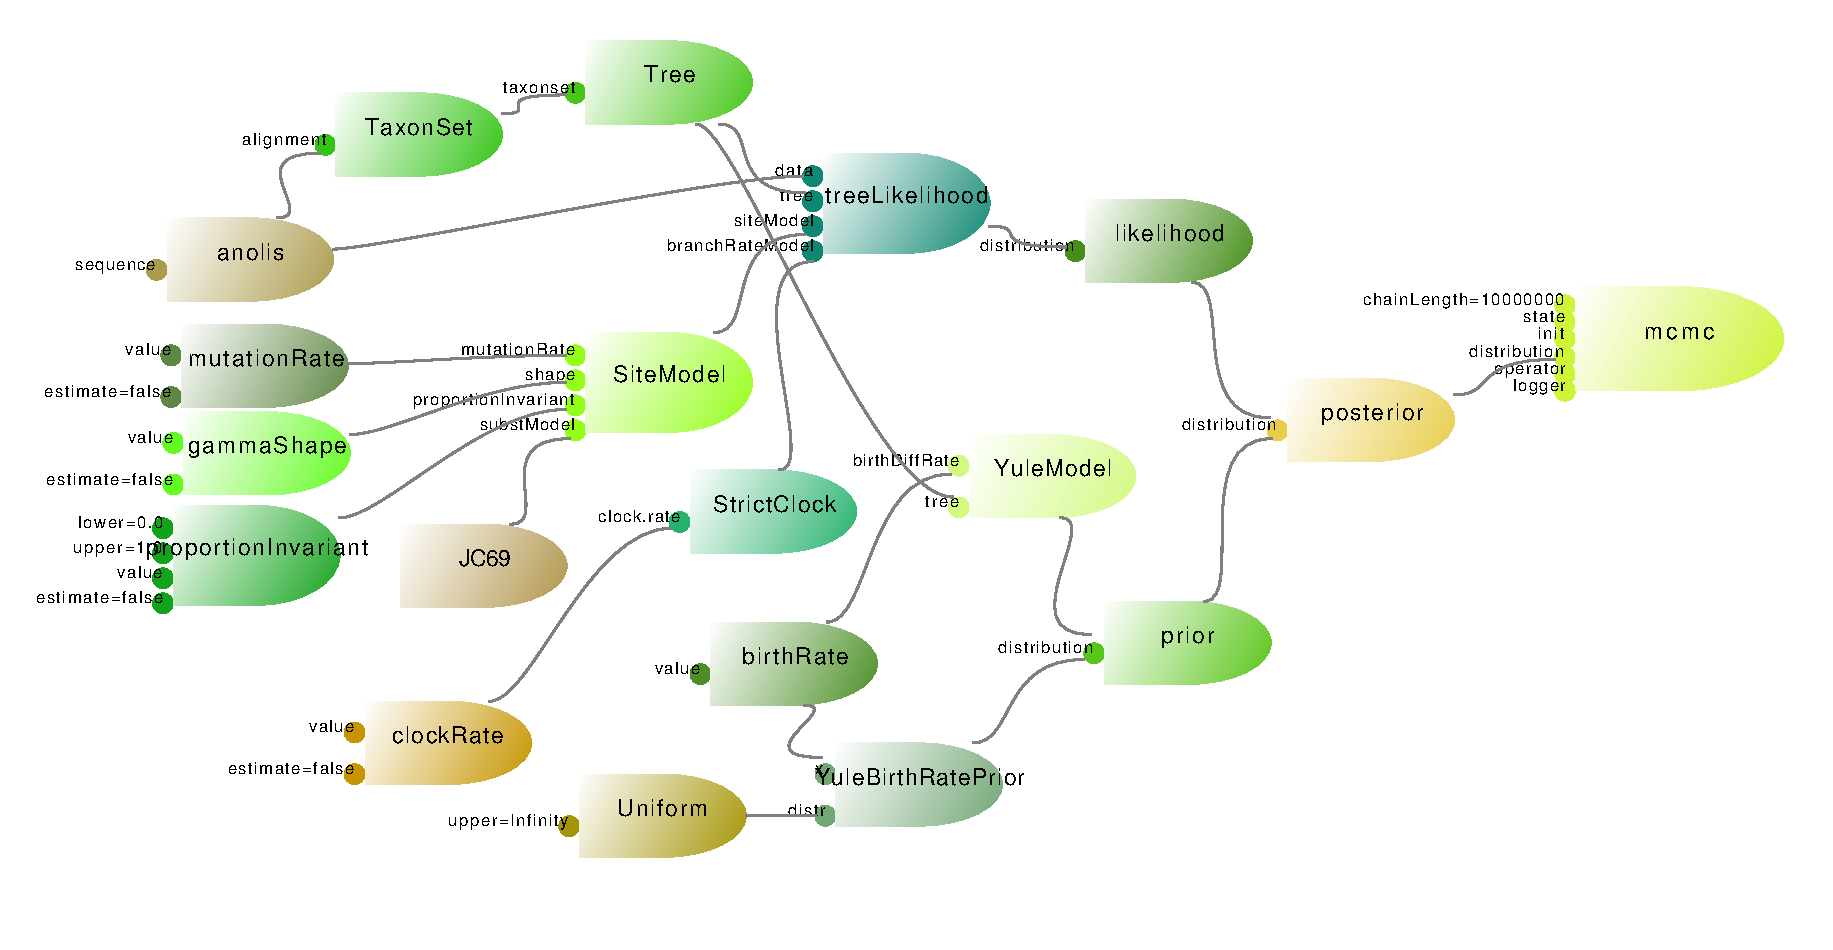
\includegraphics[width=0.8
\textwidth]{model}
\end{center}
\caption{\label{fig.model}Fragment of a BEAST model}
\end{figure}

\section{BEASTShell}

BEASTShell is based on BeanShell\footnote{\url{http://www. beanshell. org}}, which was
designed to be a dynamically typed scripting language with a Java-like syntax and
tight integration with Java. This means for Java developers that there is no need to learn 
another syntax and also that all the familiar Java libraries are directly available.

However, BeanShell by itself does not solve the issue with instantiating BEAST Objects.
Therefore, BeanShell is extended such that when creating BEASTObjects instead of calling
a constructor, it initialises all inputs with their named values and calls initAndValidate
after that to ensure the object is in an initialised state. 
The following code fragment shows Java left and the much more intuitive BEASTShell on the 
right
\begin{verbatim}
	Plot plot = new Plot();                plot = new Plot(x=xData, y=yData);
	plot.xInput.setValue(xData);
	plot.yInput.setValue(yData);
	plot.initAndValidate();
\end{verbatim}
Thus, we get the advantage
of BEASTObjects outlined above, together with the convenience of BEASTShell for constructing 
and scripting. Furthermore, a large number of commands for mathematical functions and 
statistical distributions are provided. The addition of 2D plotting and tree drawing 
algorihtms completes BEASTShell.
%
These seemingly small chances make a range of tasks a lot easier, such as
setting up simulations studies for hierarchical clustering models and
interactive exploration of properties of hierarchies produced by a BEAST 
analysis. A number of BEAST specific classes are provided where BEASTShell scripts
can be used to define the functionality of these classes. This is especially useful
for logging specific properties of the model during an MCMC run, such as functions
of some of the parameters or trees. Also, it makes it easy to specify new models 
and MCMC proposals without having to provide Java package. One of the features of BEAST
is that an analysis can be stored in fairly readable XML format so that an analysis can
be reproduced or amended by fellow researchers. The XML is automatically specified
by a BEASTObjects and its Inputs. The classes mentioned above take the script
as their inputs, so these are part of the XML file. It takes little effort to edit
the XML file and update such scripted objects to change the analysis.

One of the nice features of an interactice interpreter is that it makes it easy to
explore the behaviour of classes, which makes it easy to create unit tests to 
guarantee quality of packages.


\begin{figure}
\begin{center}
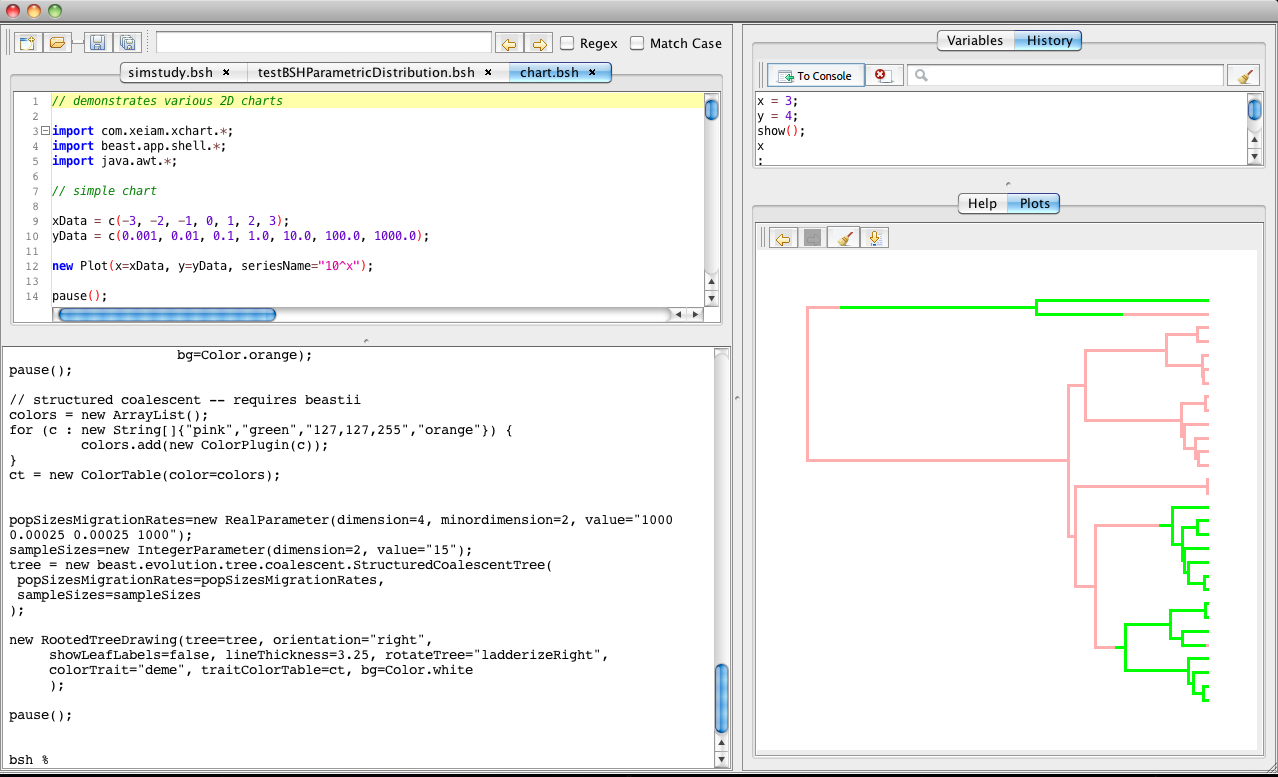
\includegraphics[width=0.9\textwidth]{BEASTStudio}
\end{center}
\caption{\label{fig.BEASTStudio}BEASTStudio -- a GUI for BEASTShell}
\end{figure}


\section{BEASTStudio -- a GUI for BEASTShell}

BEASTStudio (see Figure \ref{fig.BEASTStudio}) is inspired by RStudio \citep{rstudio}, and has similar functionality. 
It has a shell console for interactive exploration using BEASTShell, which
is equiped with tab-completion. Anything entered intot he console is added to the history displayed 
in the history pane. The history can be filtered for keywords, and portions cut and pasted into 
scripts, making it easy to run through a scenario interactively first, then compose a script around it. 
A variable inspector shows all currently available variables at present in the interpreted used by
the console, and their values can be explored.

There is an editor pane for BEAST Shell scripts, that comes with syntax colouring, 
undo/redo, search, cut/copy/paste, etc. Finally, there is a help pane, and a panel for browsing
through plots of 2D graphs and cluster hierarchies, which can be exported to bitmap
or pdf.

%\section{Documentation}

Extra attention was paid to providing documentation in the hope of decreasing
the learning curve. The help-panel in BEASTStudio contains links to various sources 
of information including BeanShell documentation updated for BEASTShell.
There are a few demos that can be run interactively in BEASTStudio, which displays the 
corresponding BEASTShell script in the console and probably provides the quickest way
to get started. The help-command can be used to show information about commands as 
well as information on BEASTObjects. Help on non-BEASObject classes is referred to
online javadocs for standard libraries. There are a few examples in the example directory,
including one for doing a simulation study.

%\section{Discussion}

\acks{Funding provided by the Royal Society of New Zealand through the Rutherford Foundation.}

\vskip 0.2in
\bibliography{bsh}


\end{document}
